\documentclass[a4paper,10pt]{article}

% Packages
\usepackage[utf8]{inputenc}
\usepackage[frenchb]{babel}
\usepackage{graphicx}
\usepackage{url}
\usepackage{hyperref}
\usepackage{a4wide}
\usepackage{amsmath}
\usepackage{../clrscode3epg}
%\usepackage{fullpage}
\renewcommand{\labelenumi}{(\alph{enumi})}

% Style
\parskip=\smallskipamount

% En-têtes
\title{
    \textbf{Structures de données et algorithmes}\\
    Répétition 1: Pseudo-code et récursion
}

\author{Gilles \textsc{Louppe} - Julien \textsc{Becker}}
\date{10 février 2012}

% Corps
\begin{document}
\maketitle

\section*{Exercice 1}

Que fait cette fonction?

\begin{codebox}
    \Procname{$\proc{Mystère}(A)$}
    \li \If $A.length < 2$
    \li \Then   \Return True
    \li \Else
    \li       \If $A[1] == A[A.length]$
    \li       \Then \Return \textsc{Mystère}($A[2..A.length-1]$)
    \li       \Else
    \li             \Return False
              \End
        \End
    \End
\end{codebox}

\section*{Exercice 2}

\begin{enumerate}
\item Ecrire le pseudo-code d'une fonction récursive permettant de calculer le $n$-ième terme de la suite de Fibonacci
\begin{align*}
F_0 &= F_1 = 1 \\
F_n &= F_{n-2} + F_{n-1} \text{ si } n > 1
\end{align*}
Réécrire ensuite cette fonction de façon itérative.

\item Ecrire le pseudo-code d'une fonction récursive permettant de calculer le $n$-ième terme de la suite de Padovan
\begin{align*}
P_{n+3} &= P_{n+1} + P_n \text{ avec } P_0 = P_1 = P_2 = 1
\end{align*}
Réécrire ensuite cette fonction de façon itérative.

\item Ecrire le pseudo-code d'une fonction itérative permettant de déterminer la valeur minimale des éléments d'un tableau. Réécrire ensuite cette fonction de façon récursive.

\item Ecrire le pseudo-code d'une fonction itérative permettant de déterminer la valeur moyenne des éléments d'un tableau. Réécrire ensuite cette fonction de façon récursive.

\end{enumerate}

\section*{Exercice 3}

Ecrire le pseudo-code d'une fonction permettant de dessiner un triangle de Sierpinski de profondeur $n$.

\begin{figure}
    \center
    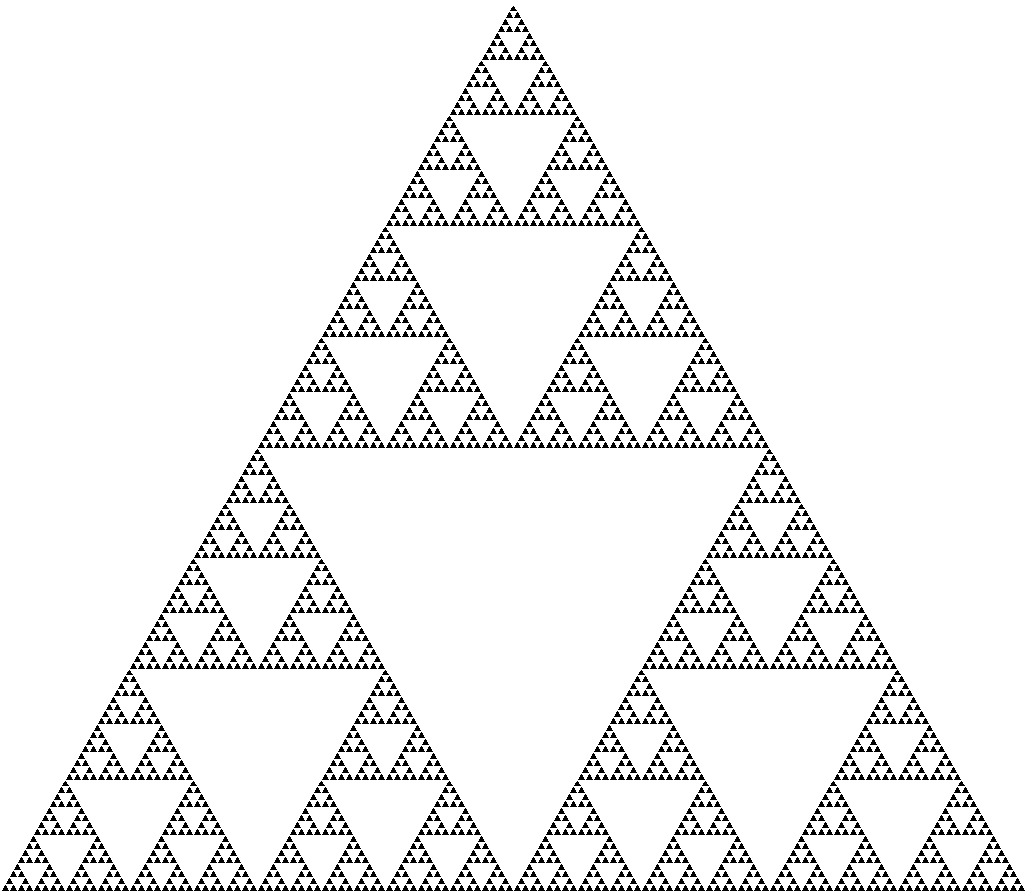
\includegraphics[scale=0.25]{triangle.png}
    \caption{Triangle de Sierpinski}
\end{figure}

\section*{Exercice 4}

\begin{enumerate}

\item Déterminer la valeur de $M(n)$ pour toute valeur de $n$.

\begin{align*}
M(n) &= \left\{
    \begin{array}{l l}
        n - 10 & \text{si } n > 100 \\
        M(M(n+11)) & \text{si } n \leq 100\\
    \end{array} \right.
\end{align*}

\item Ecrire le pseudo-code d'une fonction récursive implémentant $M(n)$.
\item Réécrire cette fonction de façon itérative.

\end{enumerate}


\end{document}
